\documentclass{article}
    % General document formatting
    \usepackage[margin=0.7in]{geometry}
    \usepackage[parfill]{parskip}
    \usepackage[utf8]{inputenc}
    \usepackage{cancel}
    \usepackage{graphicx}
    \graphicspath{./skitser/}
    % Related to math
    \usepackage{amsmath,amssymb,amsfonts,amsthm}

\begin{document}

\section{Vektorer og trigonometri}
hej


\subsection{Bevis}

\begin{proof}
    
Betragt figur \ref{fig:trekant_vektor}, hvor en vinkel $v$ er udspændt af vektoren $\vec{x}$ og $\vec{y}$.

\begin{figure}[h]
    \centering
    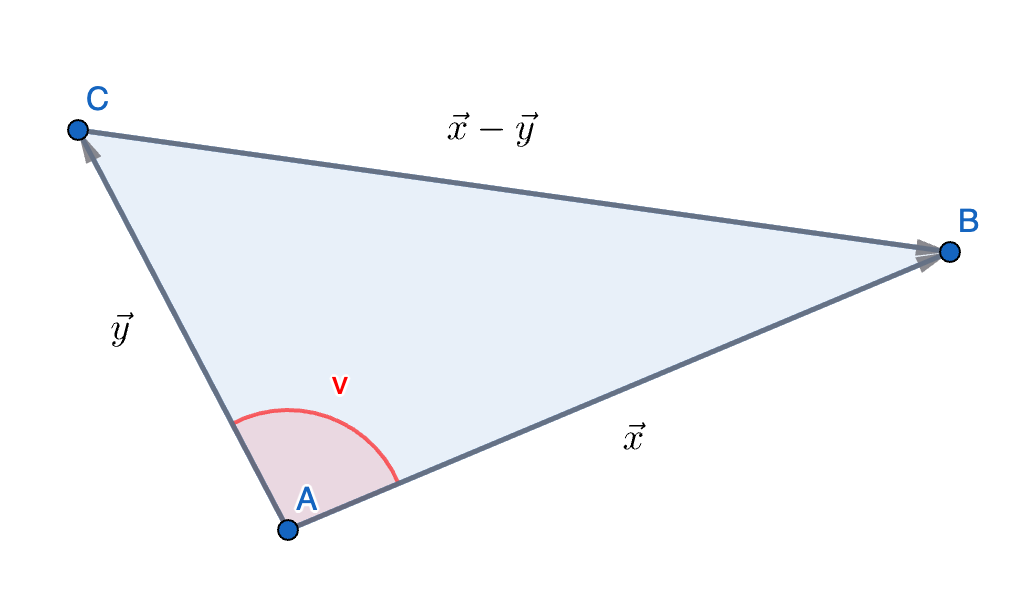
\includegraphics[scale=0.3]{./skitser/trekant_vektor_skitse.png}
    \label{fig:trekant_vektor}
    \caption{Vinkel udspændt af 2 vektorer.}
\end{figure}

Vha. af disse vektorer kan vi danne en trekant, hvori vi kan anvende cosinusrelationerne
til at lave et generelt udtryk for vinklen udspændt af 2 vektorer.
Her kan vi lave et udtryk for den lange side ved at anvende indskudsreglen:

\begin{align*}
    \vec{AB}+\vec{BC}&=\vec{AC}
    \\
    &\Downarrow
    \\
    \vec{BC}&=\vec{AC}-\vec{AB}
    \\
    &\Downarrow
    \\
    \vec{CB}&=-\vec{BC}=\vec{AB}-\vec{AC}
\end{align*}

Så den trejde side noteres $\vec{x}-\vec{y}$, og vi anvender cosinusrelationen, der siger, at i en trekant, så:

$$
    c^2=a^2+b^2-2ab \cdot \cos(v)
$$

Hvilket i vores tilfælde betyder:

$$
    |\vec{x}-\vec{y}|^2=|\vec{x}|^2+|\vec{y}|^2-2|\vec{x}||\vec{y}| \cdot \cos(v)
$$

Nu anvendes det, at $|\vec{x}|^2=\vec{x} \cdot \vec{x}$, det betyder for vores vektor:

$$
    |\vec{x}-\vec{y}|^2=(\vec{x}-\vec{y})\cdot (\vec{x}-\vec{y})
    =|\vec{x}|^2+|\vec{y}|^2-2 \cdot \vec{x}\cdot \vec{y}
$$

Det indsættes i ovenstående:

$$
\cancel{|\vec{x}|^2+|\vec{y}|^2-2} \cdot \vec{x}\cdot \vec{y}
=\cancel{|\vec{x}|^2+|\vec{y}|^2-2}|\vec{x}||\vec{y}| \cdot \cos(v)
$$

Hvor $\cos(v)$ isoleres:

$$
    \cos(v)=\frac{
        \vec{x} \cdot \vec{y}
    }{
        |\vec{x}||\vec{y}|
    }
$$
\end{proof}

\pagebreak

\section{Vektorer og linjer i planen}

\subsection{Bevis}

\end{document}
